\documentclass[xcolor=dvipsnames]{beamer}

\usepackage[utf8]{inputenc}
\usepackage{default}
\usepackage{beamerthemesplit}
\usepackage{tikz}
\usetikzlibrary{positioning,shapes,arrows}
\usetheme{Berkeley}
\usecolortheme[named=Black]{structure}

\title{Floating Base Rigid Body Dynamics Estimation}
\author{Francesco Nori, Jorhabib Eljaik}
\date{\today}


\begin{document}
% \maketitle

\begin{frame}
 \titlepage
\end{frame}

\begin{frame}
 \frametitle{Table of contents}
 \tableofcontents
\end{frame}

\section{Introduction}
\begin{frame}
  \frametitle{Sensor fusion on the iCub}
\begin{figure} 
  \centering 
	  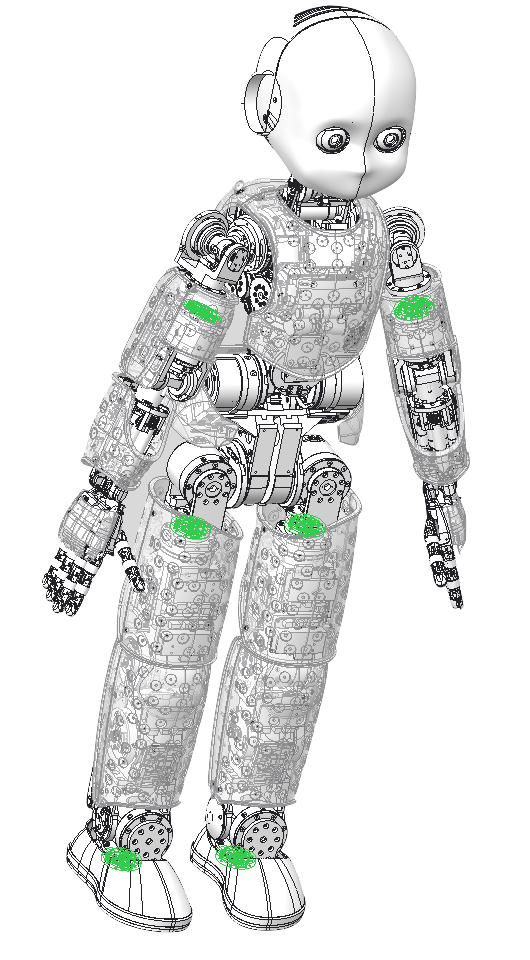
\includegraphics[height=0.55\hsize]{images/png/FT.png} 
	  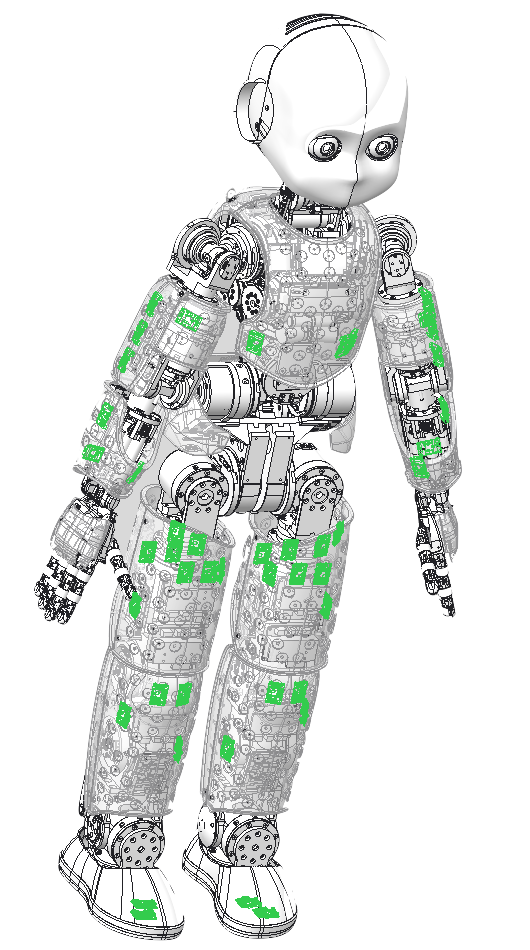
\includegraphics[height=0.55\hsize]{images/png/acc.png} 
	  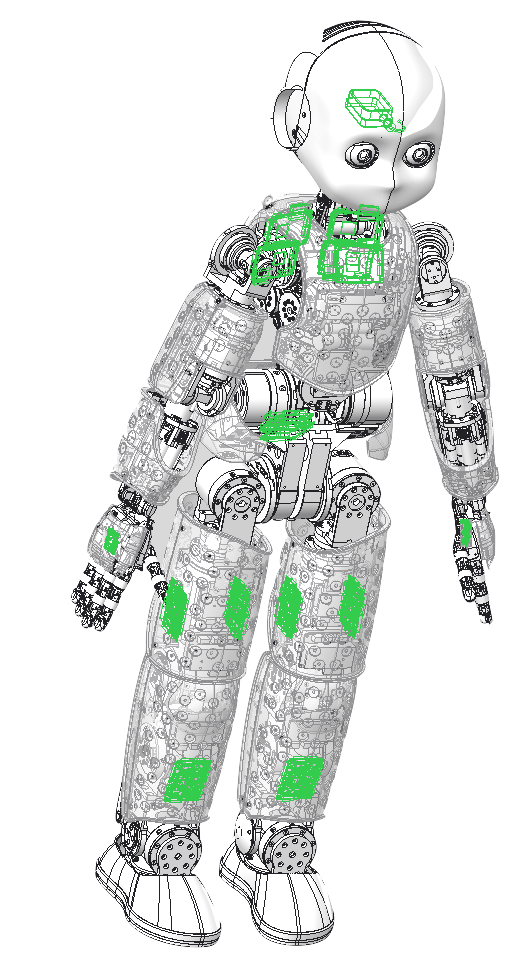
\includegraphics[height=0.55\hsize]{images/png/gyroAcc.png} 
\end{figure}
\end{frame}

\begin{frame}
  \frametitle{Sensor fusion on the iCub}
\begin{figure} 
  \centering 
	  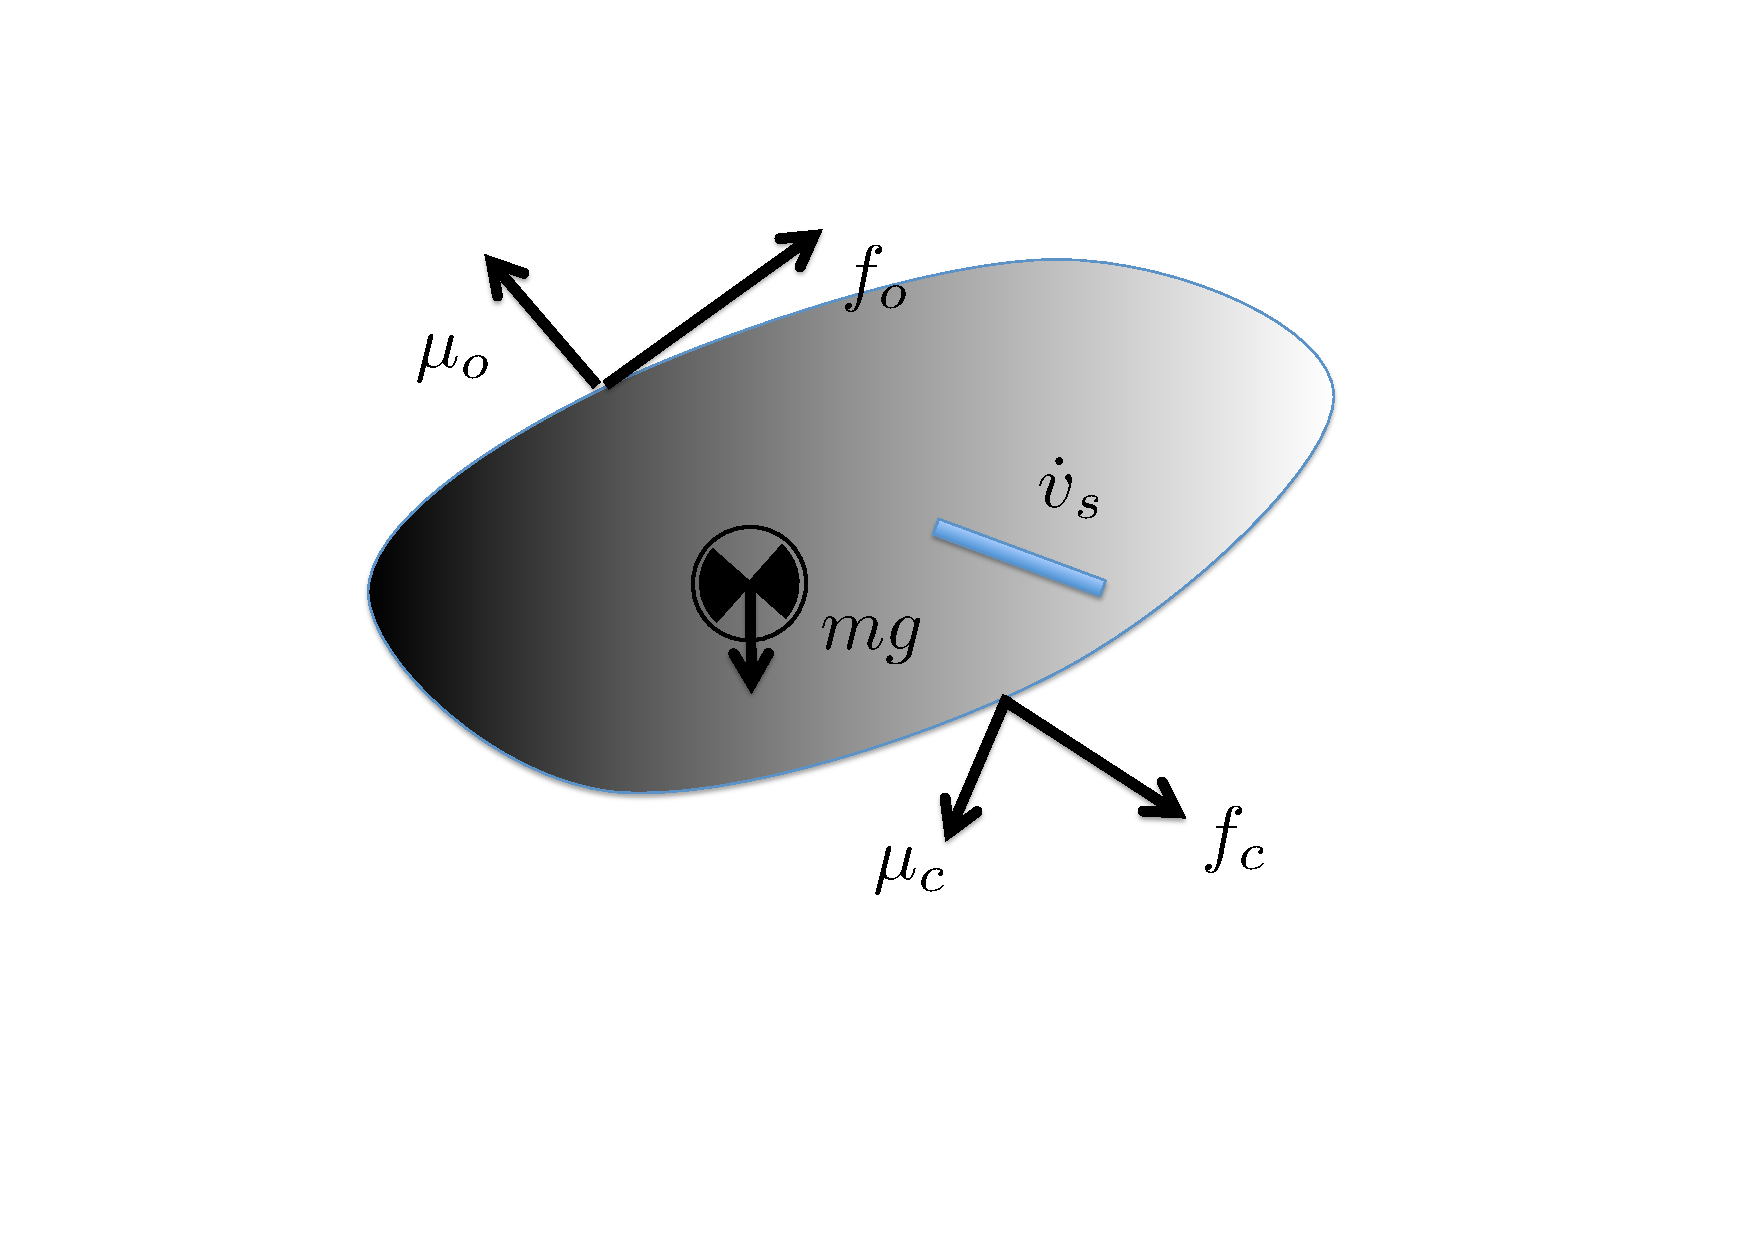
\includegraphics[height=0.55\hsize]{images/pdf/rigidBody.pdf} 
\end{figure}
\end{frame}

\begin{frame}
  \frametitle{Sensor fusion on the iCub}
\begin{figure} 
  \centering 
	  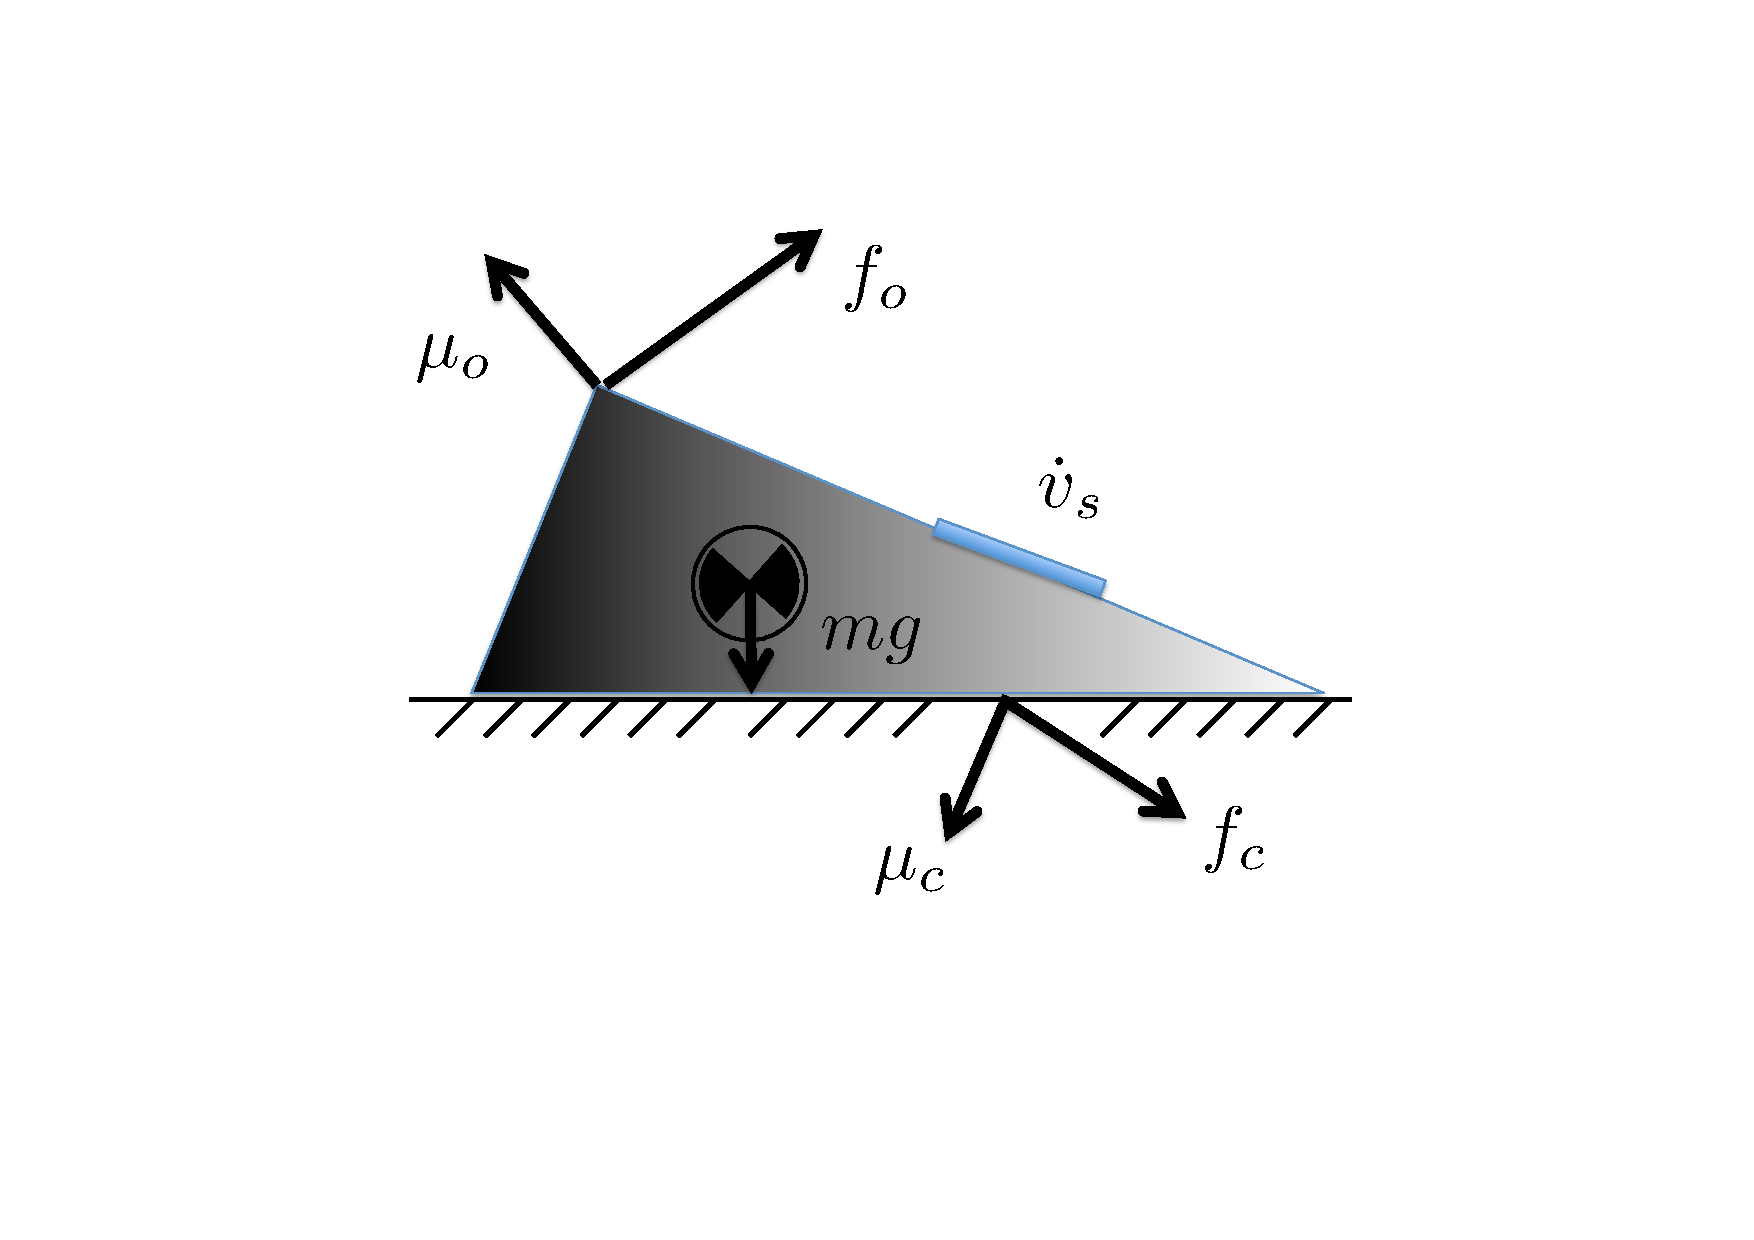
\includegraphics[height=0.55\hsize]{images/pdf/foot.pdf} 
\end{figure}
\end{frame}

\begin{frame}
  \frametitle{Sensor fusion on the iCub}
 \begin{eqnarray*}
m    \dot v^B    + \omega^B \times (m       v^B) & = & f^B_1  + ... + f^B_n + mg^B \\
I^B \dot \omega^B + \omega^B \times (I^B \omega^B) & = & \mu^B_1 + ... + \mu^B_n
\end{eqnarray*}
\begin{itemize}
\item $I^B$    : inertia in the body reference frame
\item $m$      : mass of the rigid body
\item $f^B_i$  : i-th force expressed in the body reference frame
\item $\mu^B_i$ : i-th torque expressed in the body reference frame
\item $\omega^B$: angular velocity expressed in the body reference frame
\item $v^B$    : linear velocity in the body reference frame
\item $q$      : quaternion representing the rigid body orientation
\end{itemize}
\end{frame}

\begin{frame}
  \frametitle{Sensor fusion on the iCub}
 \begin{eqnarray*}
m    \textcolor{red}{\dot v^B}    + \omega^B \times (m       v^B) & = & \textcolor{red}{f^B_1  + ... + f^B_n} + mg^B \\
I^B \dot \omega^B + \omega^B \times (I^B \omega^B) & = & \textcolor{red}{\mu^B_1 + ... + \mu^B_n}
\end{eqnarray*}
\begin{itemize}
\item $I^B$    : inertia in the body reference frame
\item $m$      : mass of the rigid body
\item \textcolor{red}{$f^B_i$}  : i-th force expressed in the body reference frame
\item \textcolor{red}{$\mu^B_i$} : i-th torque expressed in the body reference frame
\item \textcolor{green}{$\omega^B$}: angular velocity expressed in the body reference frame
\item \textcolor{red}{$\dot v^B$}    : linear acceleration in the body reference frame
\item $q$      : quaternion representing the rigid body orientation
\end{itemize}
\end{frame}

\begin{frame}
  \frametitle{Extended Kalman Filter results}
  Linear Velocities smoothing
\begin{figure} 
  \centering 
	  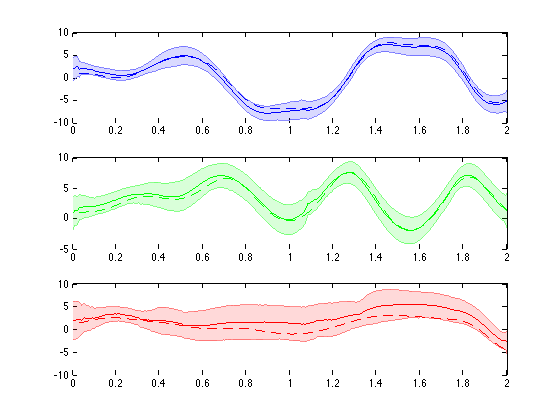
\includegraphics[height=0.70\hsize]{images/png/linVel.png} 
\end{figure}
\end{frame}

\begin{frame}
  \frametitle{Extended Kalman Filter results}
   Angular velocities smoothing
\begin{figure} 
  \centering 
	  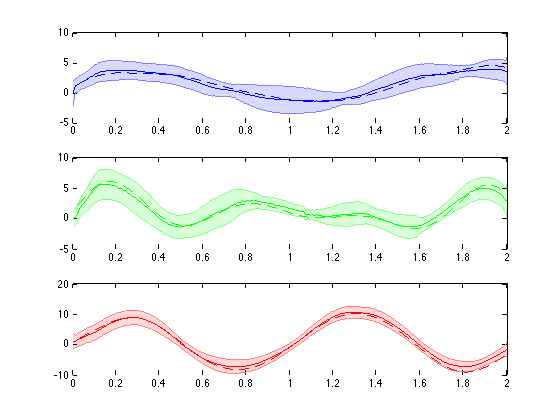
\includegraphics[height=0.70\hsize]{images/png/angVel.png} 
\end{figure}
\end{frame}

\section{Solving a Linear System with a Bayesian Network}
\begin{frame}
  \frametitle{Solving a Linear System with a Bayesian Network}
  Given a linear system $\mathbf{Ax} = \mathbf{b}$, the computation of the solution vector $\mathbf{x^*}$ is identical to the inference of the vector of marginal means $\mu = \{\mu_1, ... , \mu_n\}$ over the graph $\mathcal{G}$ with the associated Joint Gaussian Probability Density Function
  
 \begin{equation}
  p(\mathbf{x}) \backsim \mathcal{N}(\mu \triangleq \mathbf{A}^{-1}\mathbf{b}, \mathbf{A}^{-1})
 \end{equation}

 The mean of this probability distribution is the target solution. The solution of the system implies inferring the marginal densities:
 
 \begin{equation}
  p(x_i) \backsim \mathcal{N}(\mu_i = \{\mathbf{A^{-1}}\mathbf{b}\}_i,P^{-1}_i = \{\mathbf{A}^{-1}_{ii})
 \end{equation}
 
 Where $\mu_i$ and $P_i$ are the marginal mean and inverse variance.

%  Reference: Gaussian Belief Propagation Solver for Systems of Linear Equations. Ori Shental 1 , Paul H. Siegel and Jack K.   Wolf, Danny Bickson and Danny Dolev
\end{frame}



\section{The Extended Kalman Filter}
\begin{frame}
  \frametitle{The Extended Kalman Filter}
  Given a nonlinear system:
  \begin{align}
   y &= h(x) + \rho_m \\
   x_k &= f(x_{k-1}, u_{k-1}) + \rho_p
  \end{align}
  
  Where $y$, the measurement vector and $x$, the state vector have gaussian uncertainties.

  After linearizing our dynamical system about an estimate of the current state $\tilde{x}$, the corresponding Extended Kalman Filter can be obtained following a \textbf{prediction} and \textbf{update} steps.
  \begin{alertblock}{Prediction}
    $\mathbf{\tilde{x}}_k = f(\mathbf{\tilde{x}}_{k-1}, \mathbf{u}_{k-1})$
  \end{alertblock}
  
  \begin{alertblock}{\textbf{Update}}
    $\mathbf{\hat{x}}_k = \tilde{x}_k + K_k(y_k - h(\mathbf{\tilde{x}}_k))$
  \end{alertblock}

\end{frame}


\section{Update Step of the Kalman Filter as a Bayesian Network}
\begin{frame}
  \frametitle{Update Step of the Kalman Filter as a Bayesian Network}
  \textbf{Update Step} $\leftrightarrow $ \textbf{Cond. Probability of} $\tilde{x}$ \textbf{given} $y$ \\
  in other words, we can also obtain $\hat{x}$ as:
  \begin{equation}
  \mathbf{\hat{x}} = p(\tilde{x}_k \mid y_k)
  \end{equation}
  Where:
  \begin{align}
   y_k \vert_{\tilde{x}_k} \backsim \mathcal{N}(C\tilde{x}, R) \\
   x \backsim \mathcal{N}(\tilde{x})
  \end{align}

\end{frame}


\section{Bayesian Network for a Floating Base Rigid Body System}
\begin{frame}
 \frametitle{Bayesian Network for a Floating Base Rigid Body System}
 
 \begin{tikzpicture}[
  node distance=1cm and 0cm,
  mynode/.style={draw,circle,text width=1cm,align=center}
  ]
  \node[mynode] (x) {$\tilde{x}_k$};
  \node[mynode,below=of x] (y) {$y_k$};
  \path (x) edge[-latex] (y);
 \end{tikzpicture}

\end{frame}

% \section{Section no.1} 
% \begin{frame}
% \frametitle{frame title}
% Each frame should have a title.
% \end{frame}
% \subsection{Subsection no.1.1  }
% \begin{frame}
% Without title somethink is missing. 
% \end{frame}

\end{document}
